\chapter{Methodology}
In this section a performance model for understanding the runtime characteristics of deep learning models is outlined. To understand these characteristics, the underlying factors that affect it need to be understood first. 
\section{Problem Space}
The inference performance of a deep learning model is mainly affected by two major parts, the structure of the model itself and the hardware environment where it gets deployed. A third factor is the serving framework.

\subsection{Deep Learning}
Deep learning models are defined as neural networks with many layers and hidden units, the most popular being convolutional neural networks and recurrent neural networks right now, which are special forms of neural networks.
There are many different operators, which makes performance prediction very complex.
In the following the two most popular networks get analyzed.
%This increased amount of layers leads to complex mathematical calculations.
\subsubsection{Convolutional Neural Network}
This special subclass of neural network achieved wide success in the field of object recognition and detection in images. Convolutional Neural Networks (CNN)
\paragraph{Input}
The input of CNNs often consists of images, but also can be...

\paragraph{Operations}
filter, pool, 
\subsubsection{Recurrent Neural Network}
Recurrent neural networks (RNN) are made for the processing of sequences and made a lot a progress in the fields of voice recognition.
\paragraph{Input}
seqeuences
\paragraph{Operations}
GRU, LTSM
\begin{itemize}
    \item parameter von Modellen
    \item Was für Einfluss haben diese Parameter?
\end{itemize}
\subsection{Hardware Evironment}
\begin{itemize}
    \item constraints in hardware
    \item neue accelarators
    
\end{itemize}
\section{Deployment}
Model deployment describes the process of deploying a trained machine learning model to a production environment for inference purposes. 

There can be differentiated in two different deployment methods, the first one is deploying the model directly to edge devices, while the second outsources the model to a cloud-backend, where the inference is performed and the prediction is sent back to the edge device.
\subsection{Edge Deployment}
Edge devices are characterized by offering a limited amount of hardware and are often mobile, which results in a limited amount of available energy. 
Example devices are smartphones, cars or Raspberry Pis.

 

\begin{itemize}
    \item Was ist Edge (Beispiele)
    \item Was macht Edge aus?
\end{itemize}
\subsection{Cloud Deployment}
While the breakthroughs in deep learning is very interesting for AI applications on the edge devices, the computational demand needed for edge deployment often exceeds the available power to be viable.
That is why the option of outsourcing the models to a cloud-backend has becoming increasingly popular in the recent years.
Cloud-backend offer a huge amount of computational power, especially suitable for deep learning in the form of GPUs,TPUs, etc..


The big downside of cloud-based inference is the needed network connection, in particular for edge devices such as cars, where a reliable network connection can often not be guaranteed for example in rural areas. Hence this is not a viable solution for applications that are critical like autonomous driving.
\begin{itemize}
    \item Was ist cloud?
    \item Was macht cloud aus
\end{itemize}
\section{Deployment Trade-offs}

\subsection{Performance Metrics}
Several metrics are important to measure the inference performance.
\subsubsection{Inference Time}
Inference time describes the time needed from requesting a prediction from a deep learning model given an specific input until getting the prediction.
This metrics is essential for the performance, since AI application often need predictions in realtime.
\subsubsection{Energy Consumption}
This metric is particular important for mobile edge devices, since they often are powered by batteries with a limited lifespan. So if the inference process of a model consumes too much energy, the application using the model is not viable.
\subsubsection{CPU Usage}
Since the inference operation is most of the time not the only process running on a system and other processes need to run simultaneously to the inference, the CPU usage is an important metric.
\subsubsection{Memory Usage}
Similar to CPU usage, inference should not occupy the whole memory of system or even demand more memory than the available memory of a edge devices.
\subsubsection{GPU Usage}
\subsubsection{Throughput}
In order to accomplish realtime AI a high enough throughput is essential.
\begin{itemize}
    \item Unterschiede aus verschiedenen deployment optionen
\end{itemize}
Metriken:
\begin{itemize}
    \item Welche Metriken (inference time....)
    \item Wie werden die Metriken gemessen?
    \item Wo werden Metriken gemessen?
\end{itemize}
\begin{figure}[H]
\centering
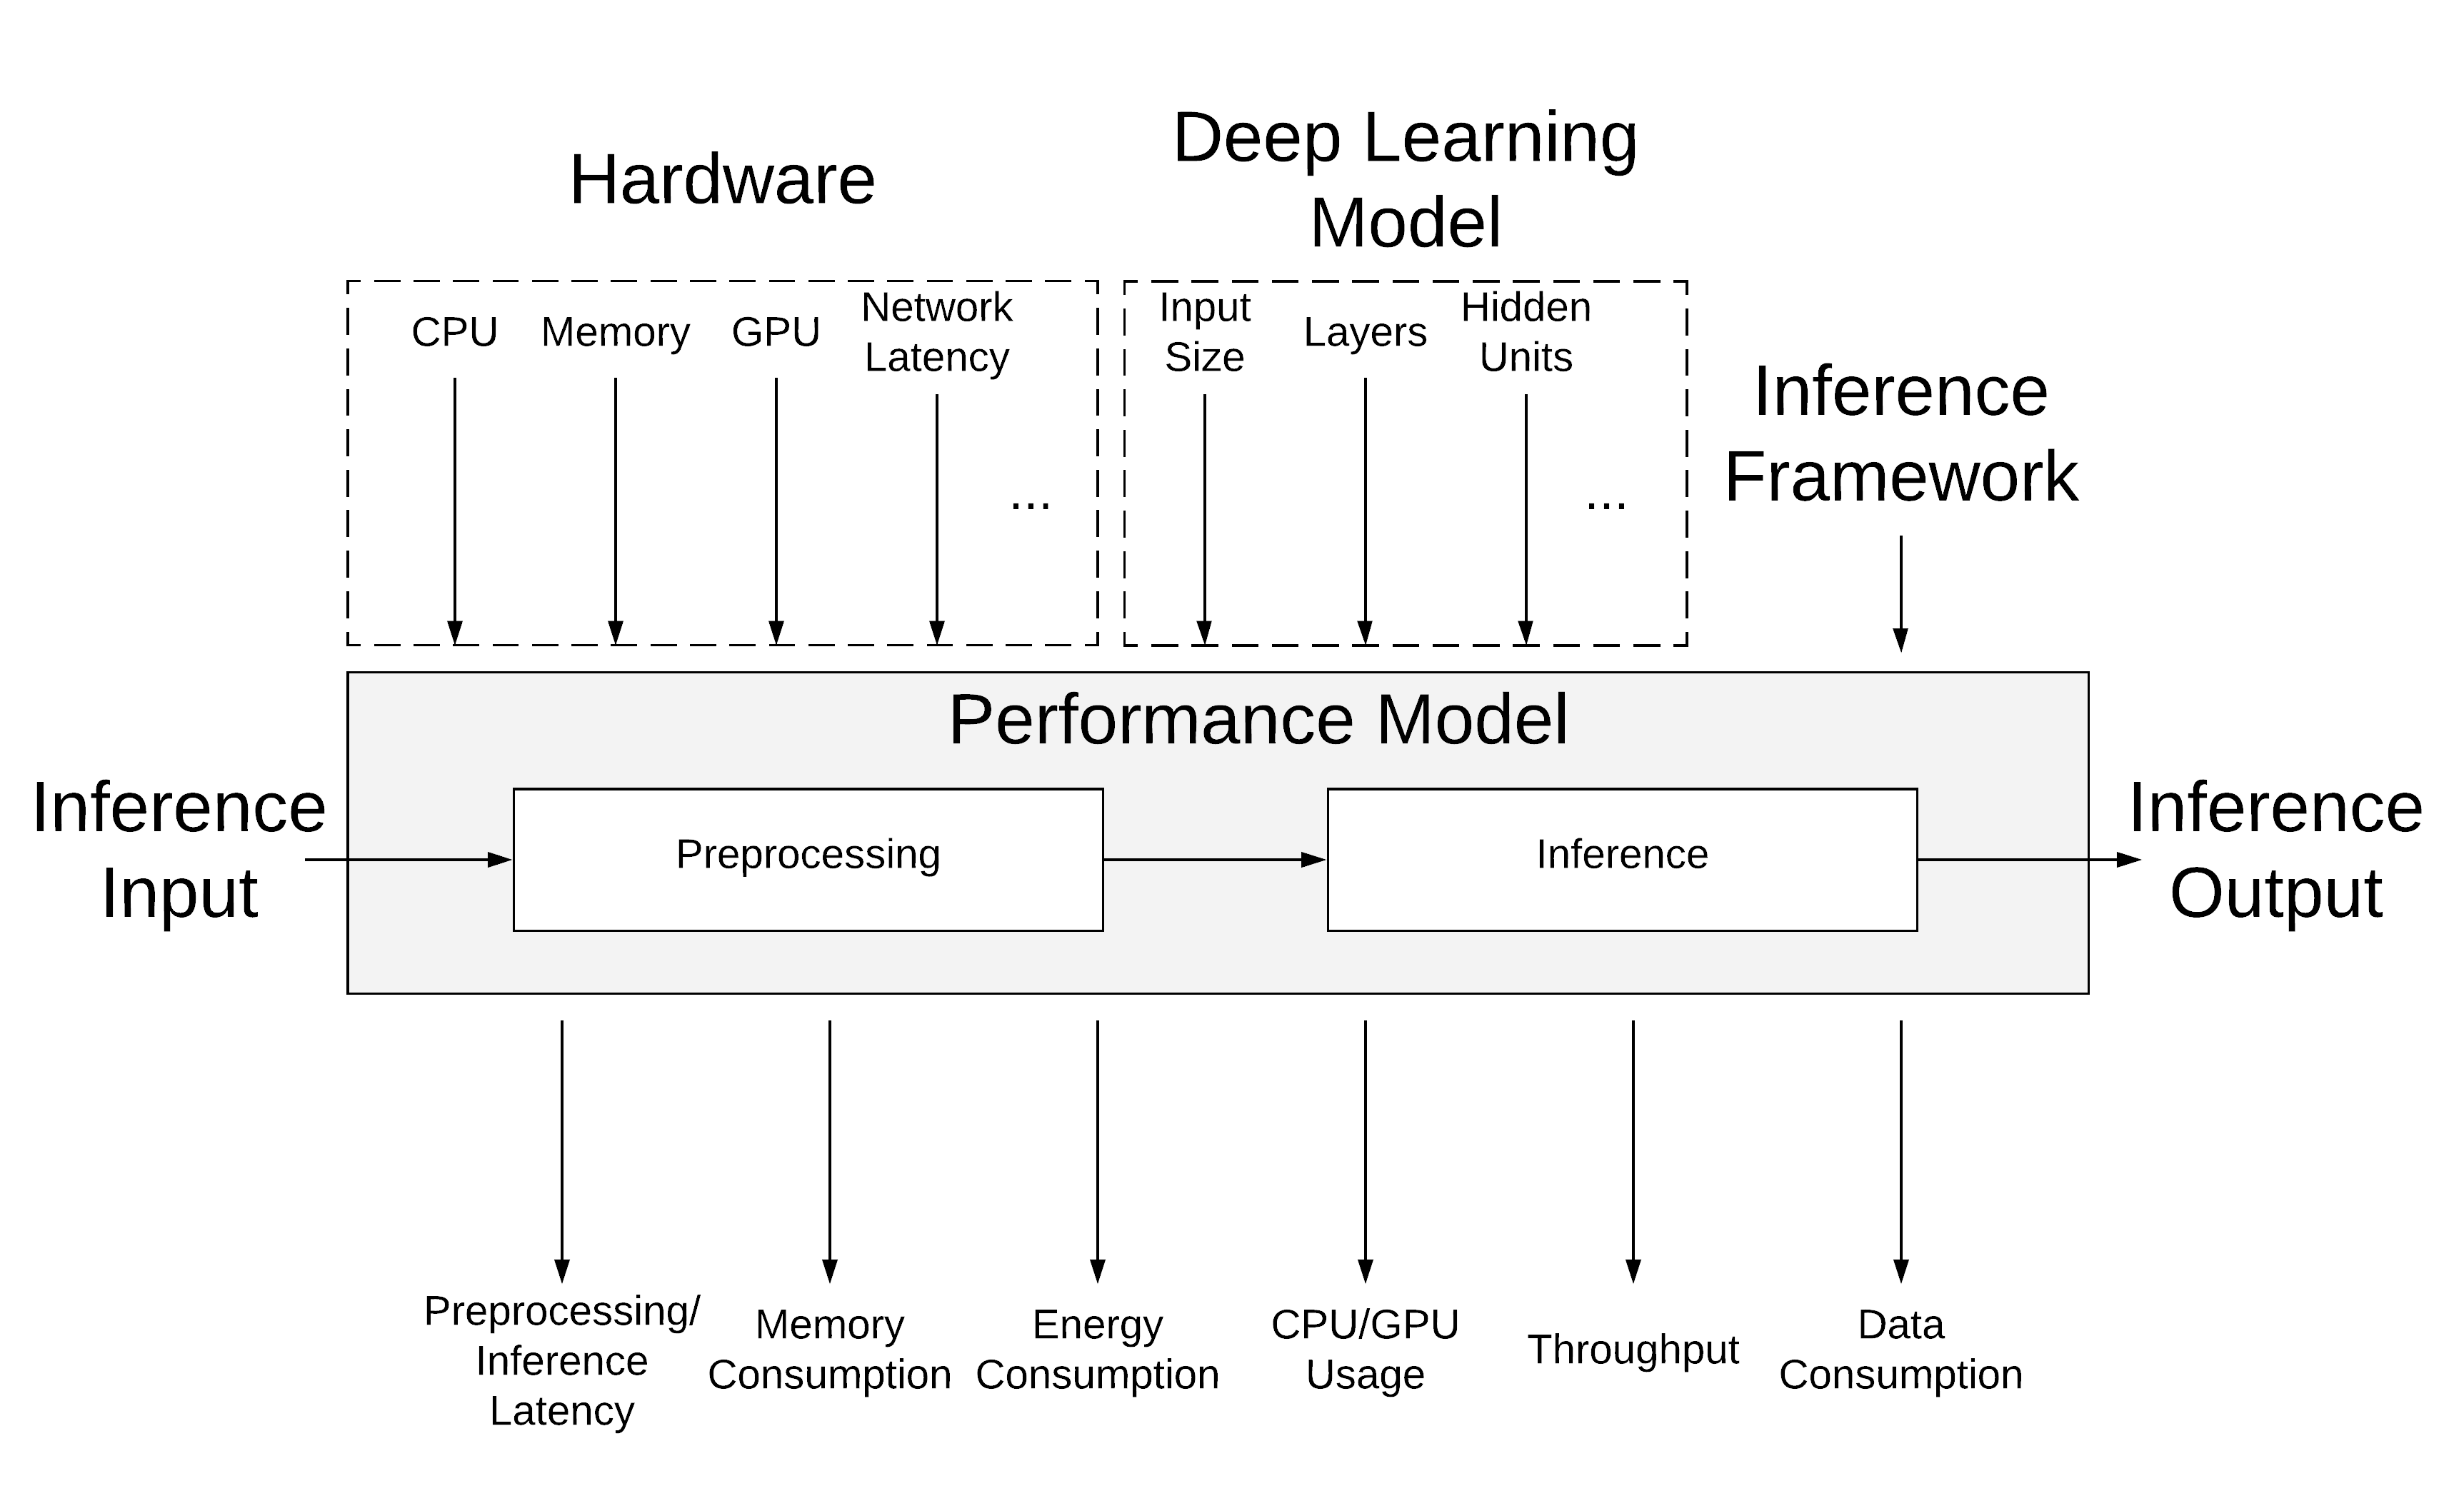
\includegraphics[width=0.9\textwidth]{./Bilder/trade_offs.png}
\caption{Performance Model}
\label{fig:perf_model}
\end{figure}
\endinput 